\subsubsection{Huấn luyện mô hình từ dữ liệu thời tiết}
Task 5 tập trung vào việc xây dựng một pipeline hoàn chỉnh để huấn luyện mô hình trên máy tính, chuyển đổi mô hình sang định dạng phù hợp cho vi điều khiển và triển khai suy luận trực tiếp trên ESP32-S3. Quy trình này được thể hiện rõ trong tệp \texttt{TFL\_For\_MCU.py} thuộc thư mục \texttt{prism-uploads}. Điểm mạnh của cách làm này là toàn bộ chuỗi xử lý được tổ chức nhất quán, từ dữ liệu gốc đến mô hình cuối cùng dùng trong firmware.

Bộ dữ liệu đầu vào là tệp \texttt{weather\_classification\_data.csv}. Trong kịch bản huấn luyện, chỉ ba cột \texttt{Temperature}, \texttt{Humidity} và \texttt{Weather Type} được giữ lại để phục vụ bài toán phân loại. Đây là một lựa chọn phù hợp với định hướng TinyML, bởi mô hình càng ít đặc trưng đầu vào thì càng nhẹ và càng dễ suy luận nhanh trên phần cứng hạn chế tài nguyên.

Trước khi huấn luyện, dữ liệu được làm sạch bằng phương pháp \textit{Interquartile Range} (IQR) nhằm loại bỏ ngoại lai ở hai cột nhiệt độ và độ ẩm. Từ 13.200 mẫu ban đầu, sau bước lọc còn lại 13.108 mẫu hợp lệ. Các nhãn dự đoán được mã hóa thành bốn lớp \texttt{Cloudy}, \texttt{Rainy}, \texttt{Snowy} và \texttt{Sunny}, với phân bố khá cân bằng giữa các lớp. Việc cân bằng dữ liệu như vậy giúp giảm nguy cơ mô hình thiên lệch về một nhóm thời tiết cụ thể.

\subsubsection{Tiền xử lý và cấu trúc mạng}
Sau bước làm sạch, dữ liệu được chia theo tỉ lệ 80\% cho huấn luyện và 20\% cho kiểm thử, tương ứng 10.486 mẫu train và 2.622 mẫu test. Hai đầu vào nhiệt độ và độ ẩm được chuẩn hóa bằng \texttt{StandardScaler} theo công thức:

\[
x' = \frac{x - \mu}{\sigma}
\]

Trong đó, các hệ số thu được từ tập huấn luyện là:
\begin{itemize}
    \item \textbf{Nhiệt độ:} $\mu_T = 18.6480$, $\sigma_T = 16.6074$.
    \item \textbf{Độ ẩm:} $\mu_H = 68.5105$, $\sigma_H = 20.2033$.
\end{itemize}

Các hệ số này có vai trò rất quan trọng vì chúng phải được giữ nguyên khi suy luận trên ESP32. Nếu dữ liệu đưa vào vi điều khiển không được chuẩn hóa theo đúng cùng một cách như lúc huấn luyện, đầu ra của mô hình sẽ không còn đáng tin cậy.

Mô hình được xây dựng dưới dạng mạng MLP gọn nhẹ, gồm 2 đầu vào, hai lớp ẩn 16 và 8 neuron dùng hàm kích hoạt ReLU, và một lớp đầu ra 4 neuron dùng \textit{softmax}. Trong mã nguồn, mô hình được huấn luyện với bộ tối ưu \texttt{adam}, batch size 32 và 50 epochs. Cấu trúc này đủ đơn giản để chạy trên thiết bị nhúng, nhưng vẫn đủ linh hoạt để học mối quan hệ giữa nhiệt độ, độ ẩm và trạng thái thời tiết.

\subsubsection{Quy trình chuyển đổi mô hình từ \texttt{.h5} sang \texttt{.tflite} và \texttt{.h}}
Sau khi huấn luyện xong, mô hình Keras trước hết được lưu lại dưới dạng \texttt{TinyML.h5}. Đây là định dạng thuận tiện để lưu trữ đầy đủ kiến trúc mạng và trọng số, phù hợp cho giai đoạn phát triển trên máy tính. Tuy nhiên, tệp \texttt{.h5} chưa thể dùng trực tiếp trên vi điều khiển.

Bước tiếp theo là dùng \texttt{TFLiteConverter} để chuyển mô hình sang định dạng TensorFlow Lite và tạo ra tệp \texttt{TinyML.tflite}. Đây là phiên bản rút gọn, phù hợp hơn cho môi trường nhúng nhờ kích thước nhỏ và cơ chế suy luận tối ưu cho thiết bị biên. Trong dự án hiện tại, tệp này có kích thước khoảng 3 KB, nhỏ hơn đáng kể so với \texttt{TinyML.h5} ban đầu. Sau đó, kịch bản chuyển đổi tiếp tục đọc nội dung nhị phân của \texttt{TinyML.tflite}, đổi từng byte sang dạng thập lục phân và sinh ra tệp header để nhúng vào firmware. Trong phiên bản tích hợp hiện tại, phần dữ liệu mô hình được sử dụng thông qua tệp \texttt{toanvinh\_model.h}, trong đó mô hình được lưu dưới dạng mảng hằng số C để chương trình ESP32 có thể nạp trực tiếp khi khởi tạo TensorFlow Lite Micro.

Điểm đáng chú ý là phần header của mô hình cũng ghi rõ số lớp và tên các lớp dự đoán, giúp việc tích hợp với firmware dễ hiểu hơn. Vì vậy, Task 5 không chỉ dừng ở bước huấn luyện mô hình, mà còn hiện thực hóa đầy đủ quy trình đóng gói mô hình từ môi trường Python sang môi trường C/C++ nhúng.

\subsubsection{Triển khai mô hình trên ESP32}
Phía firmware, tệp \texttt{tinyml.h} trong thư mục \texttt{uploads} cho thấy mô hình được sử dụng thông qua các thành phần \texttt{TensorFlowLite\_ESP32}, \texttt{MicroInterpreter} và \texttt{AllOpsResolver}. Đồng thời, file này cũng bao gồm \texttt{toanvinh\_model.h}, cho thấy đây là tệp mô hình thực tế đang được liên kết vào chương trình. Phân hệ TinyML được đóng gói thành hai phần chính: \texttt{setupTinyML()} để khởi tạo mô hình và \texttt{tiny\_ml\_task()} để thực hiện suy luận trong lúc hệ thống đang vận hành.

Chu trình suy luận trên ESP32 có thể tóm tắt như sau:
\begin{enumerate}
    \item Đọc nhiệt độ và độ ẩm từ cảm biến.
    \item Chuẩn hóa hai giá trị này bằng đúng các hệ số đã sinh ra từ \texttt{StandardScaler} ở giai đoạn huấn luyện.
    \item Ghi dữ liệu đã chuẩn hóa vào tensor đầu vào của mô hình.
    \item Thực thi suy luận bằng TensorFlow Lite Micro.
    \item Đọc vector xác suất đầu ra và chọn lớp có xác suất lớn nhất làm kết quả dự đoán cuối cùng.
\end{enumerate}

Ưu điểm lớn nhất của hướng triển khai này là hệ thống không cần gửi dữ liệu thô lên máy chủ để phân loại. Toàn bộ quá trình nhận biết trạng thái thời tiết diễn ra ngay trên thiết bị, giúp giảm độ trễ, giảm phụ thuộc mạng và thể hiện rõ tính chất AI at the edge của đề tài.

\subsubsection{Kết quả hiển thị trên giao diện web}
Sau khi mô hình được nhúng vào ESP32, kết quả suy luận trước hết được biểu diễn trên giao diện web dưới dạng nhãn thời tiết cuối cùng. Cách hiển thị này phù hợp với người dùng vận hành, vì họ chỉ cần nắm được trạng thái dự đoán mà không cần quan tâm đến chi tiết nội bộ của mô hình.

\begin{figure}[H]
    \centering
    
\includegraphics[width=0.34\textwidth]{pictures/task5_web_prediction.png}
    \caption{Kết quả dự đoán thời tiết của mô hình TinyML trên giao diện web}
\end{figure}

Việc đưa trực tiếp nhãn dự đoán lên giao diện web giúp hệ thống tiến thêm một bước so với một mô hình đo lường thông thường: không chỉ hiển thị dữ liệu thô, mà còn cung cấp thông tin đã được xử lý để hỗ trợ người dùng ra quyết định nhanh hơn.

\subsubsection{Kiểm chứng bằng log terminal}
Bên cạnh giao diện web, hệ thống còn xuất log chi tiết ra terminal để phục vụ quá trình kiểm thử kỹ thuật. Nội dung log bao gồm giá trị đầu vào từ cảm biến, dữ liệu sau chuẩn hóa, xác suất của từng lớp và nhãn dự đoán cuối cùng. Đây là kênh rất quan trọng để xác nhận rằng mô hình sau khi chuyển đổi từ \texttt{.h5} sang \texttt{.tflite} rồi sang \texttt{.h} vẫn giữ được logic suy luận nhất quán.

\begin{figure}[H]
    \centering
    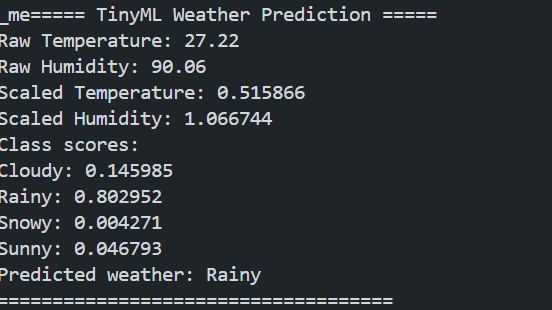
\includegraphics[width=0.68\textwidth]{pictures/task5_terminal_prediction.png}
    \caption{Log terminal của mô hình TinyML khi chạy trên ESP32-S3}
\end{figure}

Thông qua log terminal, người phát triển có thể kiểm tra được toàn bộ chuỗi xử lý nội bộ của mô hình thay vì chỉ nhìn vào kết quả cuối. Đây là bằng chứng thực nghiệm quan trọng cho thấy mô hình không chỉ chạy được trong môi trường Python mà còn hoạt động ổn định sau khi được chuyển đổi và nhúng vào hệ thống nhúng.